
\documentclass[14pt]{beamer}

\mode<presentation>
{
    \usetheme{default}
    \usecolortheme[RGB={0,150,200}]{structure}
    %\usefonttheme{professionalfonts}
    \setbeamertemplate{footline}{
        \hbox{
            \begin{beamercolorbox}[wd=.70\paperwidth,ht=4.25ex,dp=3ex,left,leftskip=2ex]{title in head/foot}%
                %\usebeamerfont{title in head/foot}\insertshorttitle{}
            \end{beamercolorbox}%
            \begin{beamercolorbox}[wd=.20\paperwidth,ht=4.25ex,dp=3ex,center]{date in head/foot}%
                %\usebeamerfont{date in head/foot}\insertshortdate{}
            \end{beamercolorbox}%
            \begin{beamercolorbox}[wd=.10\paperwidth,ht=4.25ex,dp=3ex,right,rightskip=2ex]{date in head/foot}%
                \insertframenumber{} / \inserttotalframenumber
            \end{beamercolorbox}%
        }
    }
}

\setbeamersize{text margin left=14pt,text margin right=14pt}

\beamertemplatenavigationsymbolsempty
\usepackage[czech]{babel}
\usepackage[utf8]{inputenc}
\usepackage{lmodern}
\renewcommand*\familydefault{\sfdefault}
\usepackage[T1]{fontenc}
%\usepackage{pdfsync}

\colorlet{todo}{red}
\newcommand{\todo}[1]{{\color{todo} {[[#1]]} }}

\usepackage{pifont}
\newcommand*\tick{\item[\ding{51}]}
\newcommand*\fail{\item[\ding{55}]}

\usepackage{setspace}
\setstretch{1.3}


\title[Souběžné učení v~koevolučních algoritmech]{\vskip0.5cm{}Souběžné učení\\v~koevolučních algoritmech}

\author[Bc. Michal Wiglasz]{Bc. Michal Wiglasz\\
  {\vskip1cm\footnotesize
  Vedoucí: Ing. Michaela Šikulová
}}
\date{}


\begin{document}

\begin{frame}
    \titlepage
\end{frame}


% \begin{frame}{\insertshorttitle{}}

%     \begin{enumerate}
%         \item Seznamte se s problematikou evolučních algoritmů spojených s učením, genetického programování, koevolučních algoritmů a evolučního návrhu obrazových filtrů.

%         \item Navrhněte program umožňující provádět evoluční návrh obrazových filtrů s využitím koevoluce prediktorů fitness. Velikost prediktorů fitness adaptujte v průběhu koevoluce jako reakci na konvergenci fitness při vývoji kandidátních filtrů.
%     \end{enumerate}

% \end{frame}


\begin{frame}{\insertshorttitle}
    \begin{itemize}
        \item Evoluční algoritmy:
        \begin{itemize}
            \item Genetický algoritmus.
            \item Kartézské genetické programování.
            \item Koevoluční algoritmy.
            \item EA spojené s učením.
        \end{itemize}
        \item Evoluční návrh obrazových filtrů:
        \begin{itemize}
            \item Koevoluce s prediktory fitness.
            \item Adaptovat velikost prediktorů fitness na konvergenci fitness evoluce kandidátních filtrů.
        \end{itemize}
    \end{itemize}
\end{frame}


\begin{frame}{Evoluční návrh obrazových filtrů}
    \center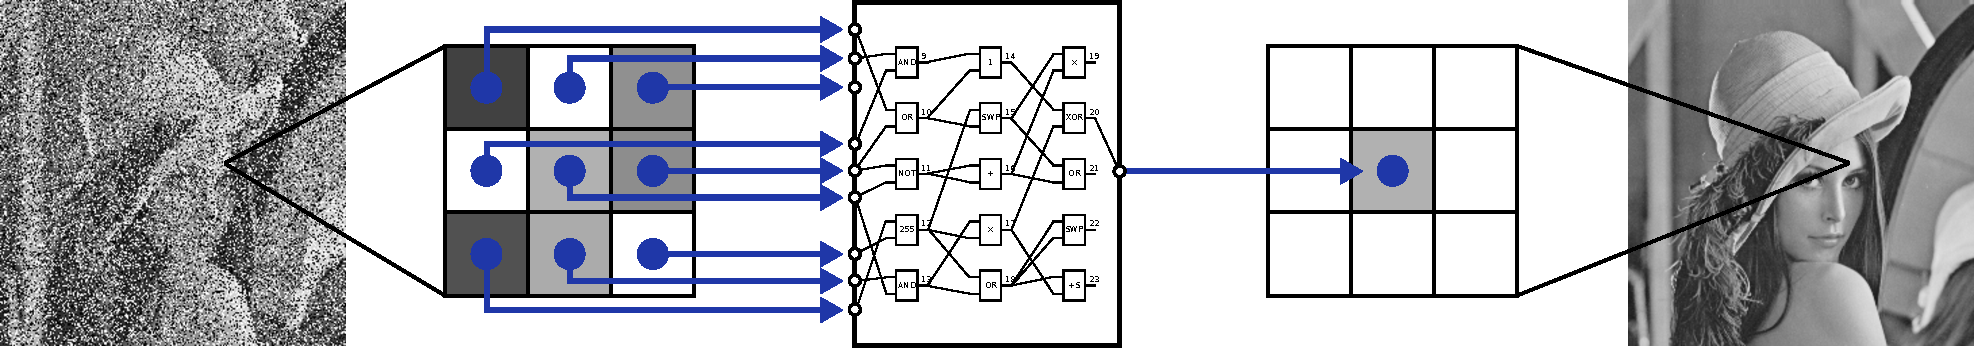
\includegraphics[width=0.95\textwidth]{fig/filter-cgp.pdf}
\end{frame}


\begin{frame}{Koevoluce s prediktory fitness}
    \center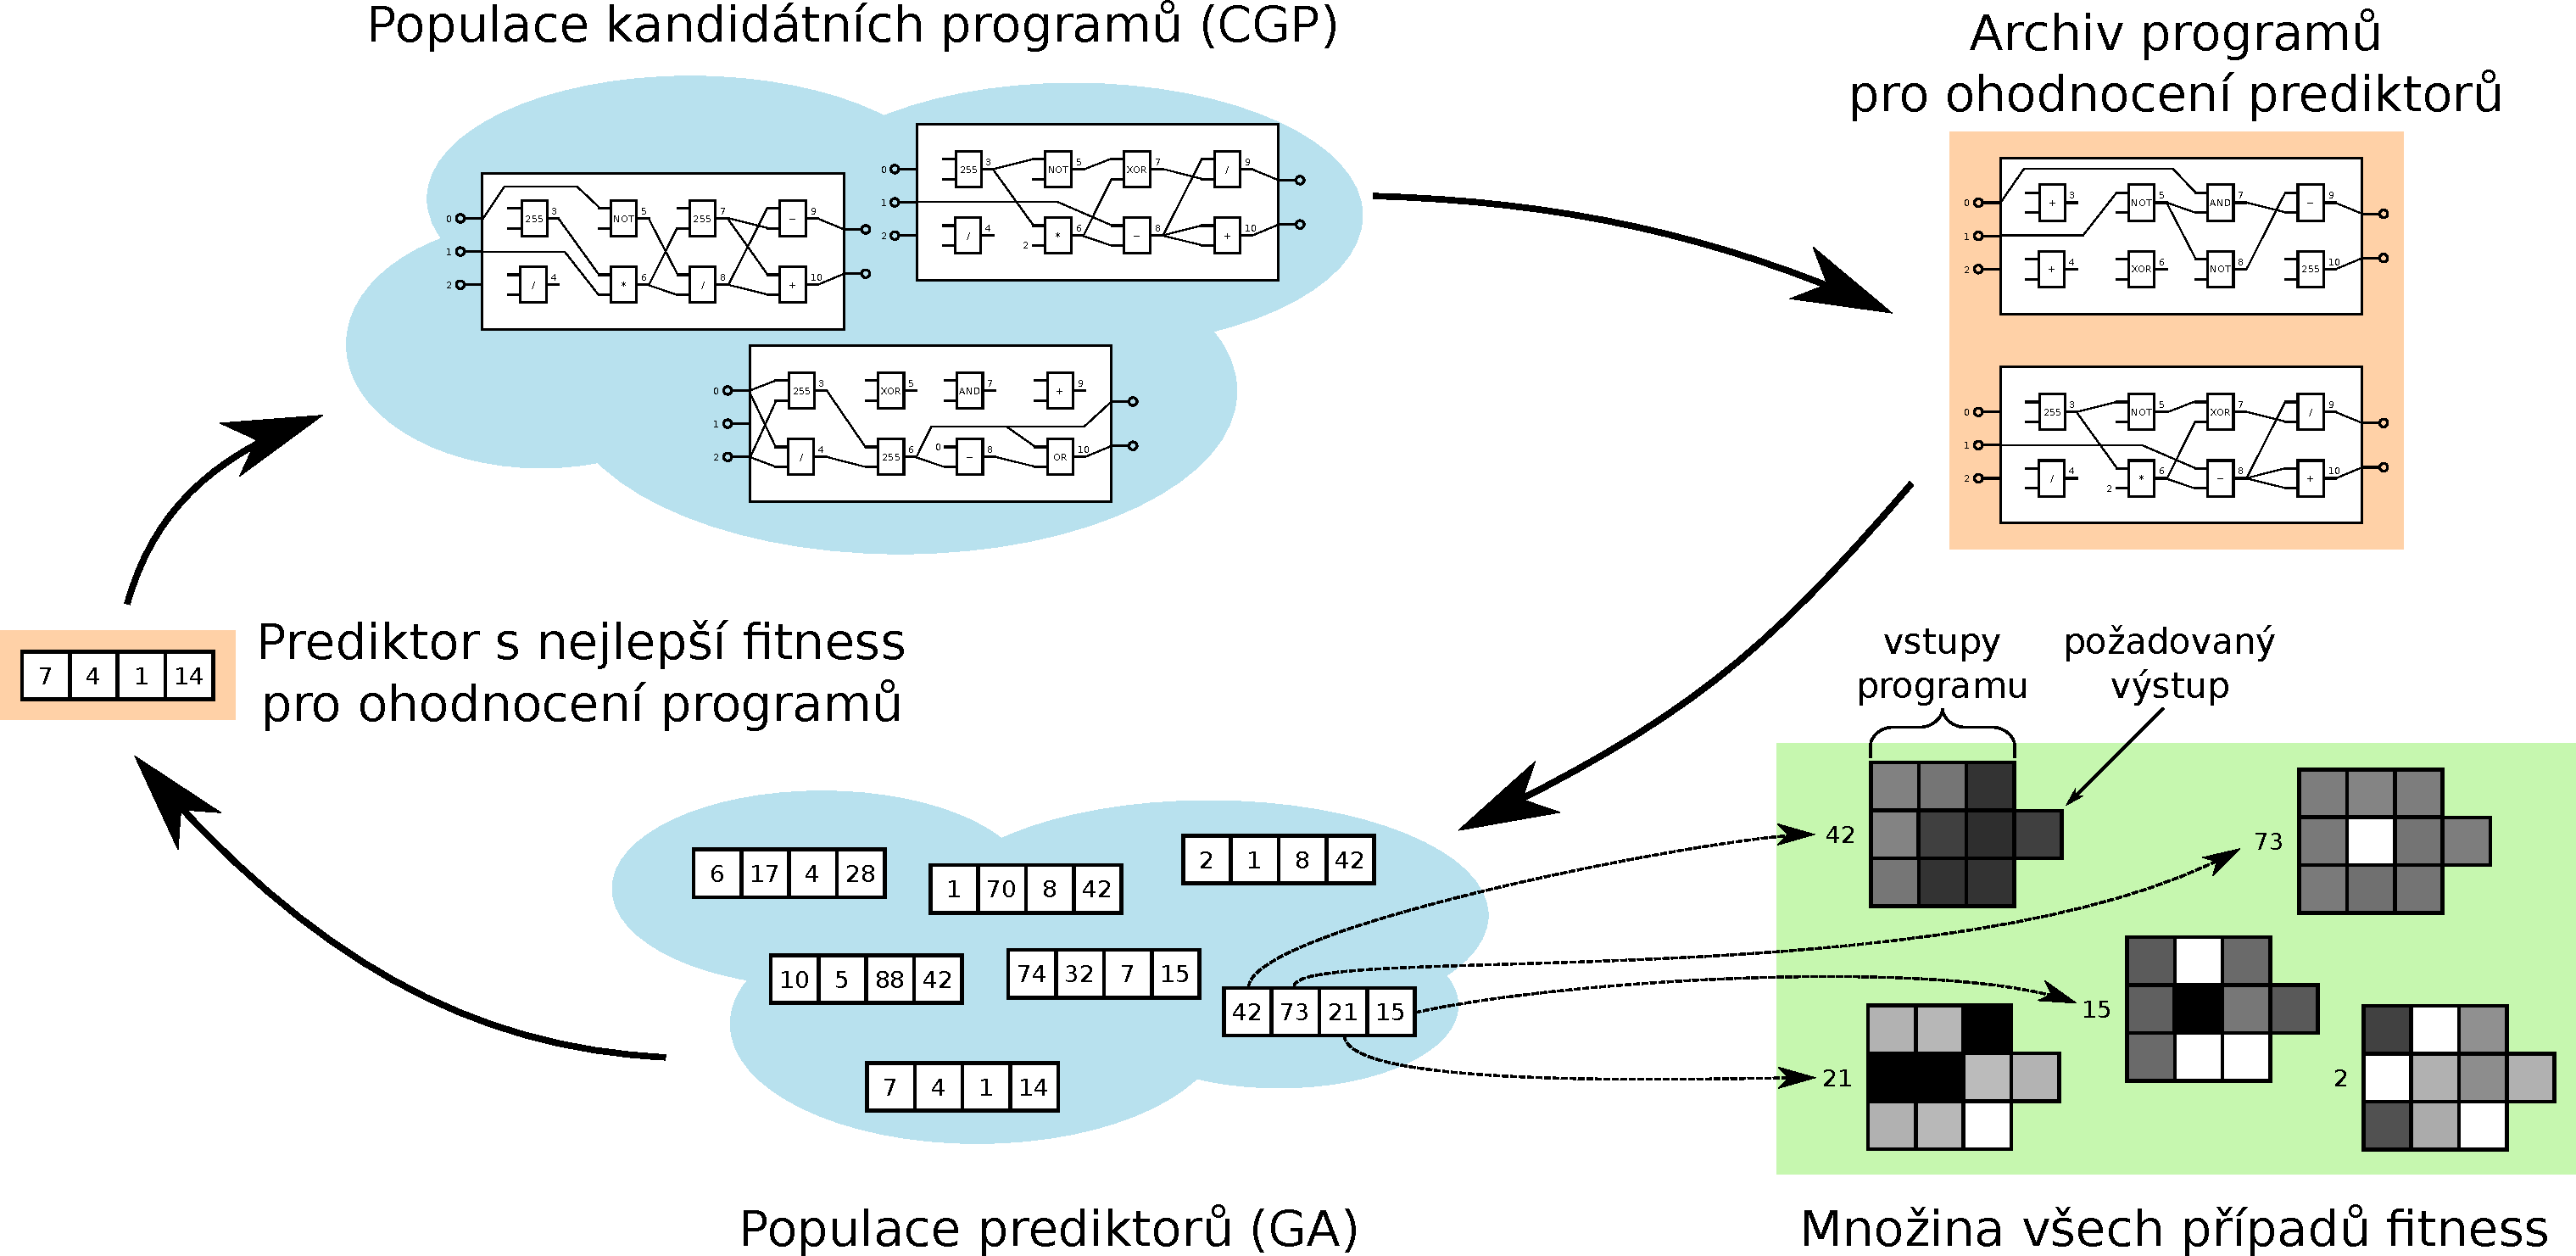
\includegraphics[width=0.95\textwidth]{fig/coevolution-if.pdf}
\end{frame}


\begin{frame}{Souběžné učení}
    \begin{itemize}
        \item Plasticita fitness
        \begin{itemize}
            \item Jedinec se snaží co nejlépe využít své geny.
            \item Adaptace jedince na prostředí.
            \item Stejný genotyp, různé fenotypy.
        \end{itemize}

        \item Různá míra plasticity:
        \begin{itemize}
            \item Mezi jedinci v populaci.
            \item Během života jedince.
        \end{itemize}
    \end{itemize}
\end{frame}


\begin{frame}{Nové kódování prediktoru}
    \begin{itemize}
        \item Přináší plasticitu.
        \item Čte se jen část genů od určitého bodu (offsetu).
        \item Duplicity se ignorují.
    \end{itemize}

    \vspace{0.75cm}
    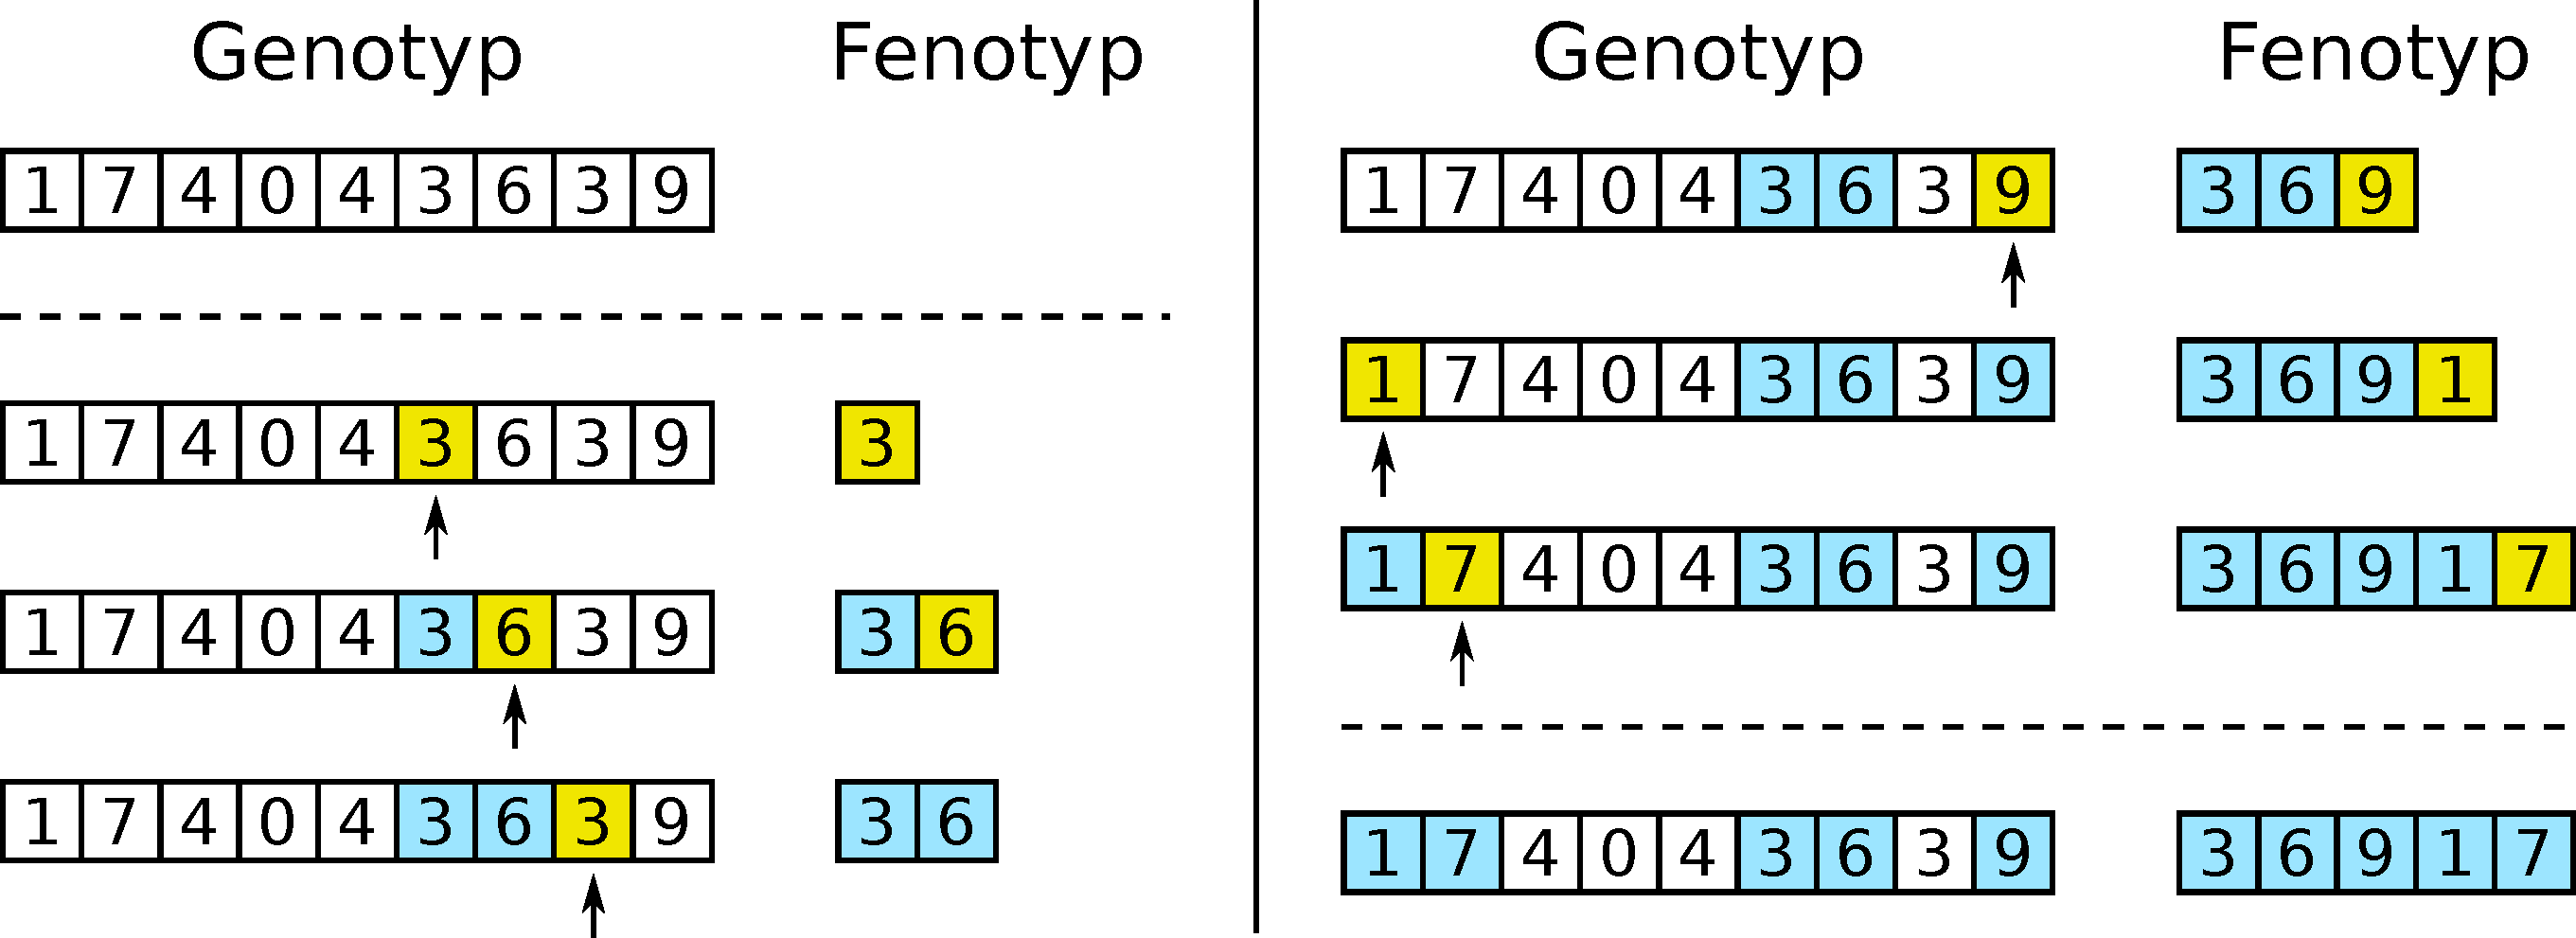
\includegraphics[width=1\textwidth]{fig/phenotype2.pdf}
\end{frame}


\begin{frame}{Nové kódování prediktoru}
    \begin{itemize}
        \item Adaptace na současný průběh evoluce.
        \begin{itemize}
            \item Podle rychlosti změny fitness se mění velikost prediktorů.
        \end{itemize}
        \item Prediktor může hledat nejvýhodnější offset.
        \item Skoková změna offsetu všech prediktorů.
    \end{itemize}
\end{frame}


\begin{frame}{Shrnutí}
    \begin{itemize}
        \item Plastický fenotyp prediktorů fitness.
        \item Adaptace na konvergenci fitness populace filtrů.
        \item Odpadá náročné hledání vhodné velikosti prediktorů.
    \end{itemize}
    \vskip1cm
    \begin{itemize}
        \item Srovnatelně kvalitní filtry, rychlejší výpočet.
    \end{itemize}
\end{frame}



% \begin{frame}{Koevoluční návrh obrazových filtrů}
%     \begin{itemize}
%         \item Obrazové filtry
%             \begin{itemize}
%                  \item Kartézské genetické programování.
%              \end{itemize}
%         \item Prediktory fitness
%             \begin{itemize}
%                 \item Genetický algoritmus.
%                 %\item \textbf{Je náročné určit nejvýhodnější velikost.}
%             \end{itemize}
%         \item Populace interagují prostřednictvím fitness:
%             \begin{itemize}
%                 \item Nejlepší obvody $\rightarrow$ fitness prediktorů.
%                 \item Nejlepší prediktor $\rightarrow$ fitness obvodů.
%             \end{itemize}
%     \end{itemize}
% \end{frame}

% \begin{frame}{Souběžné učení v evolučních algoritmech}

%     \begin{itemize}
%         \item Jedinec se snaží co nejlépe využít své geny.
%         \item Stejný genotyp, různé fenotypy -- \emph{plasticita fitness}.
%         \item \uv{Vyhlazení} fitness funkce $\rightarrow$ rychlejší konvergence.
%         %\item Učení s sebou přináší i nevýhody.
%         % \begin{itemize}
%         %     \item jedinec může zemřít,
%         %     \item je třeba udržovat učící aparát.
%         % \end{itemize}

%     \end{itemize}

%     \center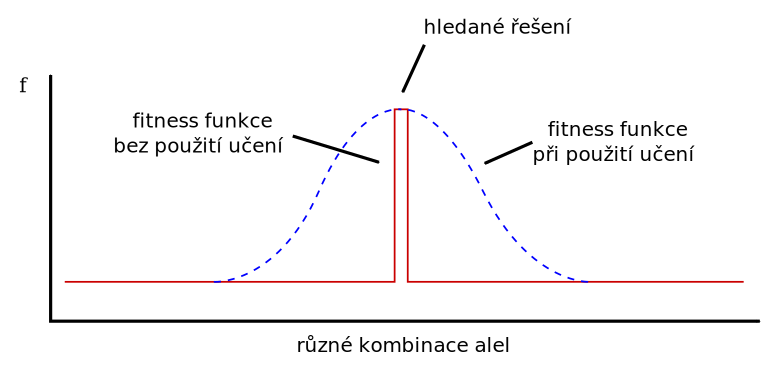
\includegraphics[height=0.5\textheight]{fig/baldwin1.pdf}
% \end{frame}

% \begin{frame}{Baldwinův efekt}

%     \begin{itemize}
%         \item Po změně v prostředí, dvě fáze:
%         \begin{enumerate}
%             \item Plastičtější jedinci jsou ve výhodě.
%             \item Naučené chování přechází do genotypu.
%         \end{enumerate}
%     \end{itemize}


%     \center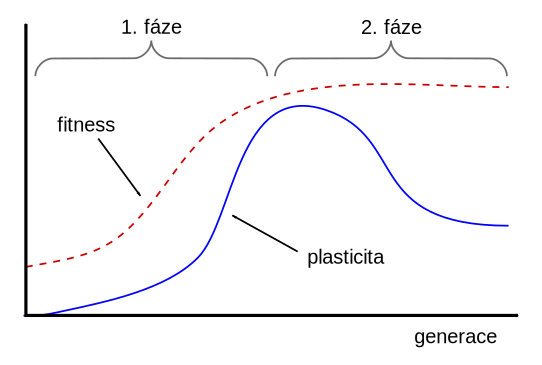
\includegraphics[height=5cm]{fig/baldwinPlasticity.pdf}
% \end{frame}

% \begin{frame}{Senzitivní období}
%     \tabularnewline
%     \begin{itemize}
%         \item Zvlášť významná fáze života jedince.
%         \item Jedinec má vyšší schopnost učení -- plasticitu.
%         \item Omezení podnětů znemožní normální vývoj.
%     \end{itemize}
% \end{frame}

% \begin{frame}{Nové kódování prediktoru}
%     \begin{columns}[T] % align columns
%         \begin{column}{.5\textwidth}

%             \begin{itemize}
%                 \item Čte se jen část genů.
%                 \item Různý počátek čtení.
%                 \item Duplicity se ignorují.
%             \end{itemize}

%         \end{column}
%         \hfill
%         \begin{column}{.5\textwidth}

%             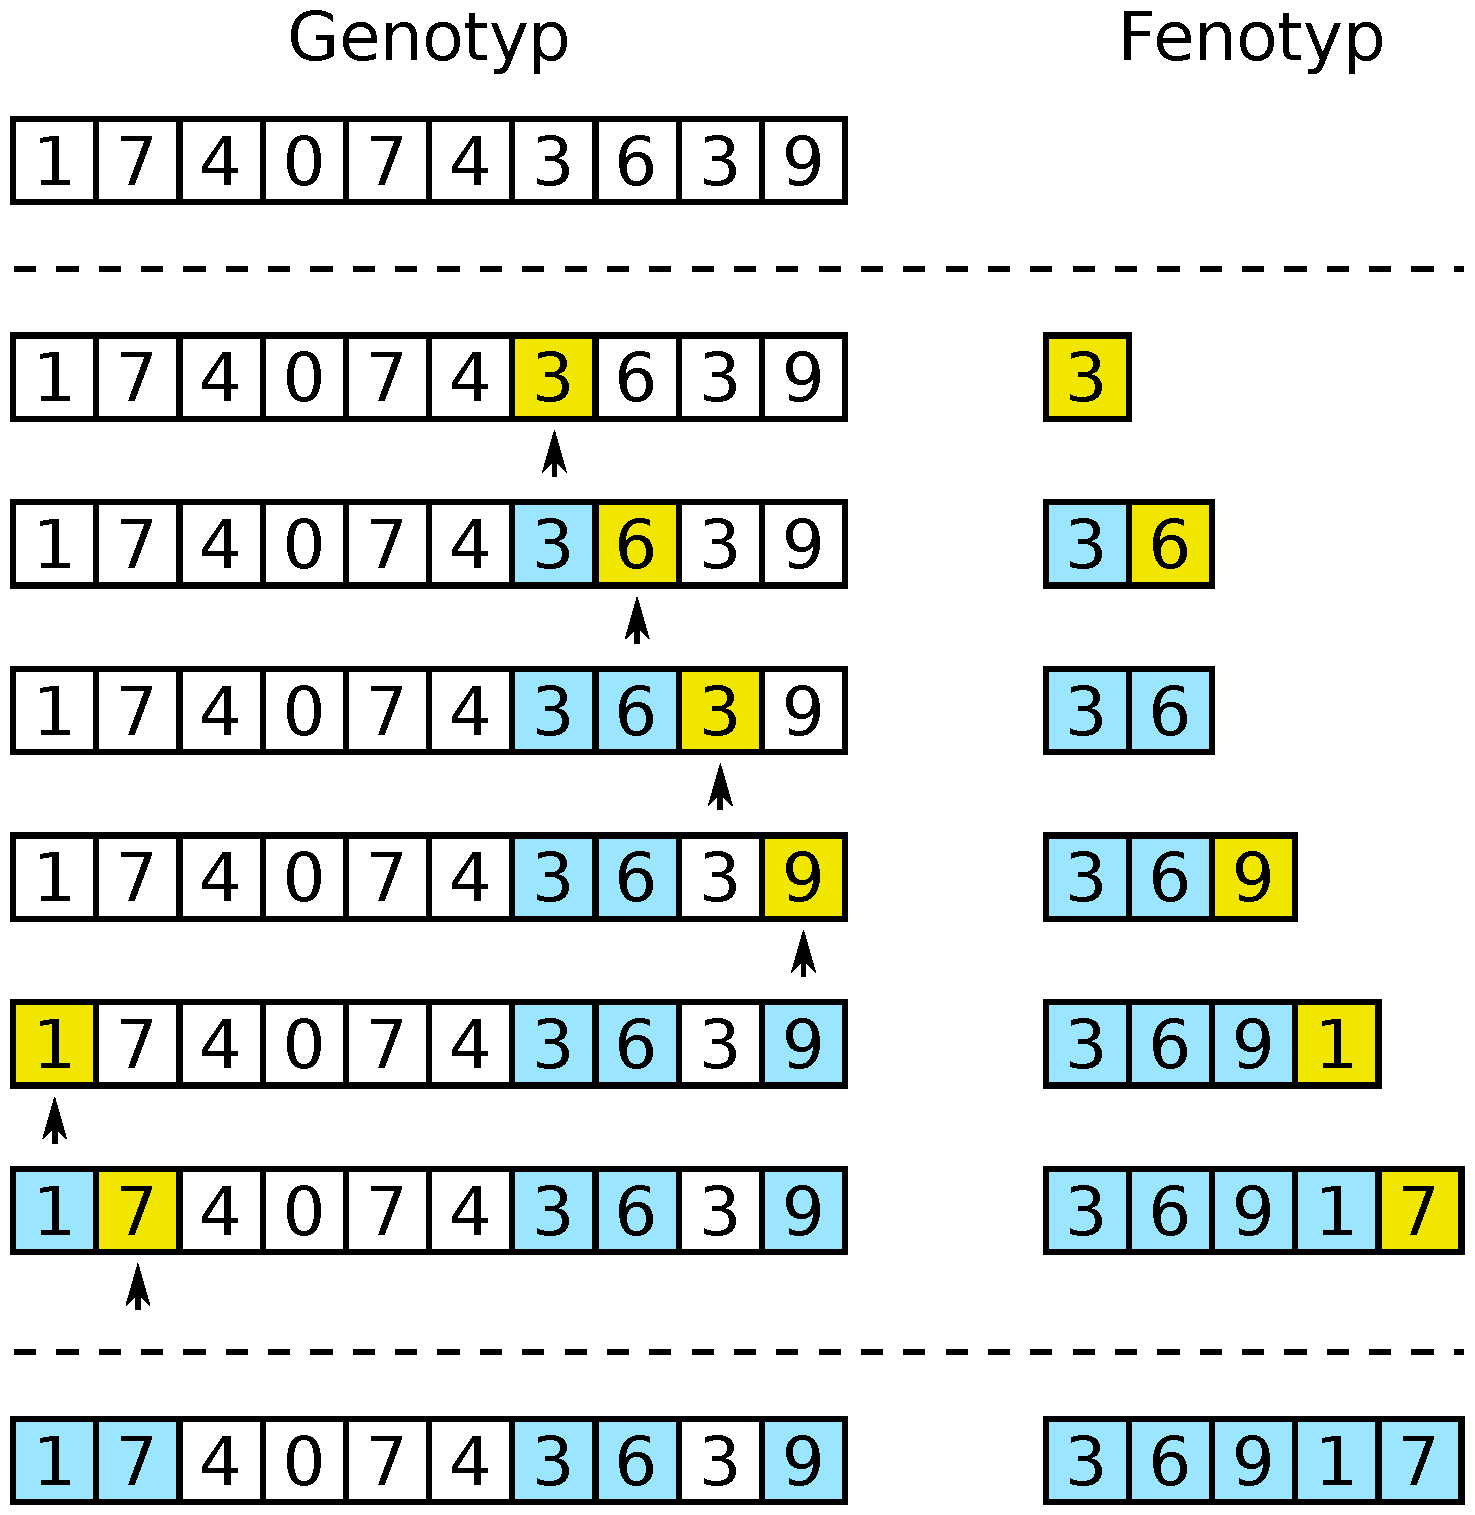
\includegraphics[width=\textwidth]{fig/phenotype.pdf}

%         \end{column}
%     \end{columns}
% \end{frame}




\end{document}



